\chapter{Introduction and Scope}

The thesis begins by defining the central diagnostic problem: terminal J--V
measurements show that a device is degrading, but they do not uniquely identify
which internal mechanism is responsible. This chapter introduces that problem,
states the research objective, and defines the scope of the COMSOL model,
experimental comparison, and supporting surrogate work.

\section{Motivation}

Perovskite solar cells (PSCs) have reached efficiencies that justify serious
reliability and manufacturing work, but their degradation remains difficult to
diagnose from external electrical measurements alone
\cite{Green_2024,Silverman_2025}. The main electrical measurement in this
thesis is the current-density--voltage curve, abbreviated as a J--V curve,
which records the current density produced by the device as the applied voltage
is swept. A measured change in J--V shape can result from ion movement,
defect-related recombination, interface changes, leakage paths, contact
resistance, or several of these effects at the same time.
Power-conversion efficiency (PCE), meaning the fraction of incident light power
converted to electrical power, reports how much performance is lost; it does
not identify the cause.

Solar cells convert absorbed photons into electrical current by generating
electron--hole pairs, separating those carriers through internal fields and
selective contacts, and collecting them at electrodes. In a perovskite solar
cell, the absorber is a metal-halide semiconductor with the general
$ABX_3$ perovskite crystal structure. Its composition can be adjusted to tune
light absorption, charge transport, and stability. Compared with crystalline
silicon, perovskites offer strong absorption in thin films, low-temperature
processing potential, lightweight or flexible form factors, and tandem-cell
opportunities. Their central limitation is operational durability under
illumination, heat, voltage bias, moisture, oxygen, and reactions at device
interfaces and electrodes.

\begin{figure}[H]
\centering
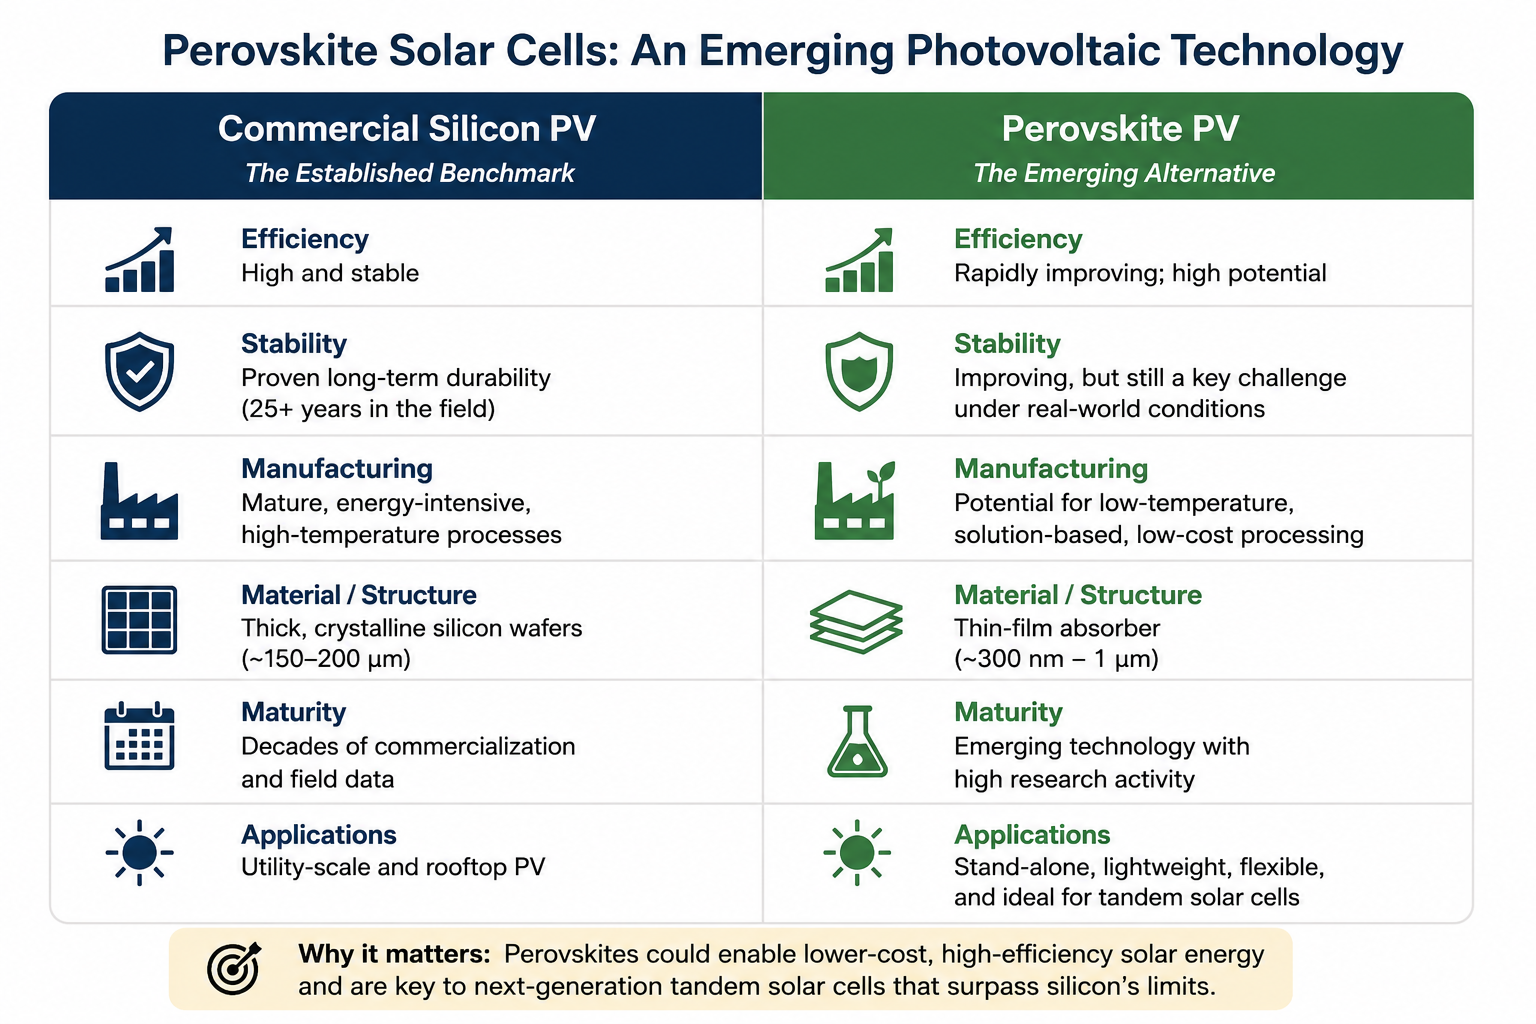
\includegraphics[width=0.92\textwidth]{figures/pptx_ai/si_vs_psc_comparison.png}
\caption{Qualitative comparison between mature commercial silicon photovoltaic
technology and emerging perovskite photovoltaics. The contrast motivates the
thesis focus: PSCs offer thin-film processing and tandem-cell potential, but
their operational stability remains the key barrier that must be understood
with device-physics and degradation modeling.}
\label{fig:si_vs_psc_comparison}
\end{figure}

This thesis develops a model in COMSOL Multiphysics, a finite-element
simulation environment, that connects measurable J--V behavior to hidden
internal mechanisms in a one-dimensional PSC stack. The model combines
electronic transport, internal electric fields, ion movement, degradation
variables, and resistance changes. Hysteresis is used in its standard PSC sense:
the measured J--V curve can depend on scan direction, scan rate, and voltage
history because internal ions and fields continue to evolve during the
measurement. The goal is not to fit one degradation curve with a trend line.
The goal is to build a model whose geometry, parameters, test conditions,
internal states, and outputs can be checked against physical expectations.

\section{Research Objective}

The objective is to develop a physics-based COMSOL model for PSC degradation
analysis. The model links observable J--V behavior to internal quantities such
as ion movement, defect growth, contact degradation, and leakage. It is
designed for future calibration against
experimental J--V, aging, impedance, transient-current, and optical data.
Impedance here means a small-signal electrical measurement that probes slow
charge, ion, and interface responses beyond a single J--V sweep. The claims in
this thesis are limited to the COMSOL model and the simulation results
reported in the following chapters.

\begin{figure}[H]
\centering
\includegraphics[width=\textwidth]{figures/pptx_ai/workflow_for_comsol_modeling_testing.png}
\caption{COMSOL modeling and testing workflow used in this thesis. A pristine
p-i-n model is compared with experimental J--V, EIS, transient-current, and
aging data; model parameters are calibrated; mobile-ion and degradation
physics are then used to predict J--V evolution and spatial state profiles.}
\label{fig:comsol_methodology_workflow}
\end{figure}

\section{Thesis Contributions}

The first contribution is a COMSOL device model based on a one-dimensional
version of the laboratory p-i-n stack. A p-i-n stack contains a p-selective
side, an intrinsic or weakly doped absorber, and an n-selective side. From the
illuminated substrate side, the physical device stack is
\begin{equation}
\mathrm{glass}/\mathrm{ITO}/\mathrm{NiO}_x/
\mathrm{MeO\mbox{-}2PACz}/\mathrm{MHP}/
\mathrm{C}_{60}/\mathrm{BCP}/\mathrm{Ag}/
\mathrm{UV\ resin}/\mathrm{glass}.
\end{equation}
Here ITO is indium tin oxide, NiO$_x$ is nickel oxide, MeO-2PACz is a
self-assembled monolayer used for hole extraction, MHP denotes the metal-halide
perovskite absorber, C$_{60}$ is fullerene, BCP is bathocuproine, and Ag is
silver.
The nominal values used in the laboratory description are approximately
30 nm NiO$_x$, 5 nm MeO-2PACz, 25 nm C$_{60}$, 4 nm BCP, 100 nm Ag, and
1.1 mm cover glass. In the COMSOL electrical model, the two hole-transport
layers are treated as one 35 nm hole-transport layer (HTL), C$_{60}$ and BCP
are treated as one 29 nm electron-transport layer (ETL), and the perovskite
absorber is 450 nm thick. ITO and Ag are the electrical contacts. Glass and UV
resin are part of the physical device, but they are not included as electronic
transport layers in the present model.
The Semiconductor Module solves the electronic device behavior, while
user-defined physics represent ion movement and gradual damage.

The second contribution is a set of degradation-mechanism parameter mappings.
The model maps hidden damage into quantities that COMSOL can use directly,
including defect density, ion charge density, series resistance, shunt
resistance, interface carrier loss, and light-generated current. Each mapping
has a physical meaning, a unit check, and an expected J--V signature.

The third contribution is a voltage-protocol method for aging and
hysteresis studies. The model separates the aging voltage
$V_{\mathrm{stress}}$ from the measurement scan voltage
$V_{\mathrm{app}}(t)$. This allows slow degradation and fast J--V scanning to
be modeled on different timescales. Multi-rate hysteretic J--V measurements are
used as calibration targets for the COMSOL degradation model.

The fourth contribution is an experimental comparison. The COMSOL
baseline and accelerated light-plus-heat degradation case are compared against
laboratory J--V data. The comparison evaluates direction, curve shape, PCE
loss, fill-factor loss, and calibration gaps rather than claiming absolute
lifetime prediction.

The fifth contribution is a first architecture-scoped stress grid for future
surrogate and inverse-model development. A surrogate model is a faster
data-driven approximation trained on COMSOL outputs, while an inverse model is
intended to infer internal device states from measured outputs. The canonical
6 $\times$ 6
light-temperature J--V sweep quantifies how accelerated aging metrics change
across coupled thermal and illumination stress. The matching profile grid
records ion, defect, recombination, electric-field, and resistance states
through the device. These outputs are not yet a final trained predictive
model, but they define the simulation data structure needed for one.

\section{Scope Boundaries}

The main thesis centers on the COMSOL model, the degradation mappings, and the
simulation results. A lightweight COMSOL-trained surrogate baseline is included
only to test whether the simulation data can train a forward model. It is not
presented as an experimentally calibrated lifetime predictor. The final claims
are therefore limited to mechanism separation within the simulated model and
to the data requirements for later calibration, inverse diagnosis, and
uncertainty analysis.

\section{Structure of the Thesis}

Chapter 2 summarizes the perovskite device physics and degradation mechanisms
needed to interpret the model. Chapter 3 defines the one-dimensional COMSOL
device geometry, material parameters, light-absorption model, ion equation, and
J--V metric extraction workflow. Chapter 4 describes the aging, hysteresis, and
transient-ion protocols used to separate slow degradation from fast electrical
measurement. Chapter 5 introduces the mappings that connect hidden defect,
contact, leakage, interface-loss, and light-generation changes to
observable J--V signatures.

Chapter 6 compares the model against experimental J--V and aging data to define
calibration targets and remaining gaps. Chapter 7 reports the simulated aging
results, electronic sensitivity sweeps, architecture-stress grid, spatial
profiles, and the lightweight COMSOL-trained surrogate baseline. Chapter 8
summarizes the limitations, reproducibility path, data availability, and future
work. The appendices collect parameter tables, mechanism mappings, and
reproducibility details so that implementation specifics do not interrupt the
main technical narrative.
